\documentclass[11pt]{article}
\usepackage[margin=1in]{geometry}
\usepackage[T1]{fontenc}
\usepackage{mathptmx}
\usepackage[table]{xcolor}
\usepackage{amsmath,amssymb}
\usepackage{graphicx,booktabs,array}
\usepackage{tikz}
\usetikzlibrary{positioning,arrows.meta}
\usepackage{hyperref}
\hypersetup{colorlinks=true,urlcolor=blue,linkcolor=black,pdftitle={PureProtX: Response to the Associate Editor and Reviewers}}
\newenvironment{excerpt}{\begin{quote}\small\sloppy}{\end{quote}}
\newcommand{\roomfor}[1]{\par\begingroup\dimen0=\pagegoal\advance\dimen0 by-\pagetotal\ifdim\dimen0<#1\baselineskip\newpage\fi\endgroup}
\newcommand{\review}[2]{\roomfor{10}\bigskip\noindent\textbf{\textit{Review #1}}\quad\textit{``#2''}\par\smallskip\hrule\medskip}
\newcommand{\reply}{\noindent\textbf{Reply:} }
\newcommand{\loc}[1]{\roomfor{7}\medskip\noindent\textbf{#1}\par\smallskip}
\newcommand{\mshead}[2]{\par\noindent\textbf{#1. #2}\par\smallskip}
\setlength{\parindent}{0pt}
\setlength{\parskip}{5pt}
\setlength{\emergencystretch}{2em}
\begin{document}
\hypersetup{pageanchor=false}
\begin{titlepage}
\centering
\vspace*{\fill}
{\Large PureProtX: A Deterministic and Verifiable Edge-Inference Framework
for IoT-Distributed Scientific Computation with Clique-Based Provenance\par}
\vspace{0.6cm}
{\large Manuscript Number: IoT-71168-2026\par}
\vspace{0.6cm}
{\large Response to the Associate Editor and Reviewers\par}
\vspace{0.6cm}
{18 October 2026\par}
\vspace*{\fill}
\end{titlepage}
\hypersetup{pageanchor=true}

\section*{To the Associate Editor}
Dear Prof. Juan Luo,

Thank you for handling our manuscript and for the decision letter dated
16 October 2026. We appreciate the Associate Editor's and reviewers'
assessment that the substantive concerns have been addressed, and the
opportunity to make the mandatory minor revisions. We have revised the
remaining claims, terminology, model inventory, and numerical explanations
to match the evidence presented.

The reviewers' comments are reproduced in italics below, followed by our
replies in regular type. Changes in the revised manuscript are shown in
\textcolor{blue}{blue}. Within each manuscript excerpt
below, text answering the current comment is blue; surrounding text and
changes associated only with other comments remain black. Shared revisions
may answer more than one comment. Locations, figure/table numbers, and
equation numbers refer to the revised manuscript, not to this response
letter; page references are PDF page positions in the compiled revision.
Reviewer~1's four unnumbered requests are numbered in their original order.

\begin{table}[!htbp]
\centering
\caption{Structural counts for the previous manuscript source and the revised manuscript.}
\begin{tabular}{lcc}
\toprule
Paper changes & Previous manuscript & Revised manuscript \\
\midrule
Number of pages & 18 & 18 \\
Number of figures & 13 & 13 \\
Number of numbered tables & 13 & 13 \\
Number of algorithms & 3 & 3 \\
Number of references & 34 & 34 \\
\bottomrule
\end{tabular}
\end{table}
% \noindent\small Source counts compare the previous manuscript at commit
% \texttt{762d36a} with the revised source. The unnumbered abbreviation
% table is excluded. The revised PDF has 18 pages; the previous PDF page
% count has not been independently established and is therefore not stated.
% \normalsize

\newpage

\review{AE}{The revision addresses the substantive concerns, and I recommend minor revision. Before acceptance, please align the claims about byte-identical re-execution, PoA$^2$, production deployment, and auditability overhead with the evidence presented. Please also clarify the missing MLP determinism results, the Merkle overhead calculation, and the score normalization and ranking convention in Eqs. (3)--(4).}


\reply We have addressed these points through a consistency review of the
manuscript and a check against the saved model inventory, benchmark results,
and scoring implementation. Table~A summarizes the corrections. In
particular, we distinguish integrity verification from configuration-dependent
exact replay, production Clique anchoring from the proposed testnet controller,
and per-record anchoring latency from percentage overhead.

\begin{center}
\textbf{Table A: Summary of the minor-revision changes.}\par\smallskip
\small
\begin{tabular}{@{}p{2.7cm}p{11.9cm}@{}}
\toprule
Issue & Change in the revised manuscript \\
\midrule
Replay scope & Restrict byte identity to validated, pinned configurations; state architecture and thread exceptions. \\
\addlinespace
Consensus and deployment & Identify production Clique; distinguish the proposed PoA$^2$ control policy and its local-testnet validation. \\
\addlinespace
Model inventory & Correct to three regressors, three classifiers, and one scaler; explain the separate synthetic MLP test. \\
\addlinespace
Overhead & Define the compute-time denominator, withdraw $<0.01\%$, and reconcile latency and speedup to archived measurements. \\
\addlinespace
Scoring and ranking & State sign reversal, bounded normalization, descending-score ranking, and the distinct CLI tie-breaking path. \\
\bottomrule
\end{tabular}
\end{center}

This round does not claim new benchmark runs. The latency figures were
regenerated programmatically from the archived CSV files, with checks of
units, per-record calculations, and speedup ratios. The revision explicitly
states the one-run scalability limitation and the different protocol for
local provenance timings. These checks establish consistency of the figures
with the archived data; they do not constitute new live-chain experiments.
Detailed replies and the corresponding manuscript excerpts follow.

\clearpage
\section*{To Reviewer \#1}
We thank the reviewer for the positive assessment of the revised evidence
and the recommendation to accept subject to the remaining corrections.
We agree that the reproducibility exceptions, the local-testnet scope of
the controller experiment, and the cost--trust distinction must also be
reflected consistently in the abstract, contributions, diagrams, and
conclusion. We address the four remaining requests below.

\review{1.1}{The manuscript still occasionally overstates heterogeneous byte-identical re-execution. The introduction/contribution language saying that `any party' can re-run on different hardware and obtain byte-identical output is broader than the actual evidence. The manuscript itself demonstrates architecture and thread-dependent exceptions. This wording should be consistently scoped to the pinned and supported configuration.}

\reply We agree. The original contribution wording was broader
than the demonstrated reproducibility envelope. We have replaced the
unconditional different-hardware claim with a requirement to reproduce a
validated, pinned execution configuration. This includes the model artifact,
runtime and dependency versions, execution provider, numeric type, and thread
settings; SVR additionally requires a compatible CPU architecture.

The manuscript now distinguishes an integrity check from a promise of
hardware-independent numerical equality: a hash comparison detects a
disagreement but cannot eliminate floating-point differences. We also correct
``three architectures'' to three devices using two architectures (x86\_64 and
aarch64). At matched thread settings, five predictive models and the scaler
agree across the tested devices; SVR is architecture-dependent, and the tree
regressors vary when thread settings change. These results do not establish
an unconditional whole-ensemble replay guarantee across architectures.
The abstract, contribution list, methodology, determinism discussion, and
conclusion have been scoped accordingly.

\loc{(a) Page 2: qualified contribution statements in Section I}
\begin{excerpt}
\mshead{I}{Introduction}

The main contributions of this work are as follows:
\begin{itemize}
\item \textcolor{blue}{We support independently verifiable re-execution
    within validated, pinned configurations. Exact replay requires
    matching model, runtime, execution provider, numeric type, and
    thread settings; SVR additionally requires the supported CPU
    architecture. Hash verification detects a mismatch rather than
    guaranteeing equivalence on arbitrary hardware.}

    \item \textcolor{blue}{We couple canonical serialization and
    on-chain artifact/result digests with explicit runtime
    configuration requirements for independent replay. The digest
    verifies integrity; configuration compatibility must also
    be established by the verifier.}
\end{itemize}
\end{excerpt}

\loc{(b) Page 13: configuration requirements and empirical scope in Section V-F}
\begin{excerpt}
\mshead{V-F}{Cross-Platform Determinism via ONNX}

\textcolor{blue}{Accordingly, an exact-replay configuration must identify
the model artifact, ORT version, execution provider, numeric type,
intra-op and inter-op thread settings, relevant dependency versions,
and CPU architecture. A verifier must reproduce the supported
configuration before expecting matching bytes; for SVR this requires
a matching architecture. At matched thread settings the other five
predictors and the scaler agree across the tested devices, including
the tree regressors despite their cross-thread differences. These
are empirical results for the tested artifacts and inputs, not a
guarantee for arbitrary hardware, models, or inputs. Hash anchoring
detects disagreement; it cannot eliminate numerical differences.}
\end{excerpt}

\review{1.2}{`PoA2' terminology remains potentially misleading. The revised manuscript admits that the underlying production chain is go-ethereum Clique and that PoA2 reliability weighting/gap control is an external proposed control layer. Therefore, statements such as `PoA2 consensus' or `PoA2-governed ledger' should be checked throughout the manuscript and precisely distinguished from the underlying Clique consensus.}

\reply We agree that the underlying block protocol and the
proposed control policy must not be conflated. The revised title identifies
Clique-based provenance. The abstract, architecture, Section~III-G,
experimental setup, consensus-results heading, provenance comparison, and
conclusion now identify the production network as stock go-ethereum Clique.
PoA$^2$ is reserved for the proposed reliability/gap-control policy.

In Section~III-G, Eqs.~(5)--(7) are explicitly introduced as a proposed policy
abstraction rather than production block acceptance or finality rules. The
production network does not implement the weighted-signature threshold in
Eq.~(5). We also relabel the approximately two-second measurement as
transaction-to-receipt latency, not ``PoA$^2$ consensus'' or finality.
Figure~2 and Table~VI are corrected on this basis; the related caption
changes are reproduced in our response to R2.4.

\loc{(a) Page 8: explicit production/policy distinction in Section III-G}
\begin{excerpt}
\mshead{III-G}{Clique Provenance and Proposed PoA$^2$ Control}
\mshead{III-G2}{Proposed PoA$^2$ Control Policy (Testnet Only)}

\textcolor{blue}{The production deployment uses stock
go-ethereum Clique, in which blocks carry individual authorized
signer seals and signer recency/voting rules govern operation.
It does not implement the weighted-signature threshold below.
We retain this equation as a proposed PoA$^2$ policy abstraction,
not a production block-acceptance or finality rule:}
\begin{equation}
\sum_{i=1}^{N_a} w_i \cdot \mathrm{sig}_i(B) \ge \theta,
\tag{5}
\end{equation}
\end{excerpt}

\loc{(b) Page 17: consistent production terminology in the conclusion}
\begin{excerpt}
\mshead{VI}{Conclusion}

\textcolor{blue}{Production anchoring uses Clique.
The proposed PoA$^2$ control layer is supported by the local
testnet failure experiment, not a production deployment claim.}
\end{excerpt}

\review{1.3}{The gap-condition mechanism should never be described as already deployed on the production PureChain network. The experiment validates it on a faithful four-signer testnet. The manuscript correctly states this in the results, but the figure and architecture descriptions should be checked for language implying production deployment.}

\reply We agree. The revised architecture distinguishes the
production anchoring path from a separate local four-signer testnet used to
evaluate the proposed controller. Neither the controller nor its reliability
weighting is presented as an already-deployed production feature. We have
checked both the figure content and the captions, rather than relying only
on a qualification in the results text.

Section~III-G states that signer-set changes were requested through Clique
voting in the local experiment. Section~V-B retains the measured testnet
failure envelope and controller timings as evidence for that experiment
only. The conclusion explicitly identifies production failure injection and
larger signer sets as future work. The production anchoring transactions
are not described as controller-deployment evidence.

\clearpage
\loc{(a) Page 5, Figure 1: architecture separates production and testnet roles}
\begin{excerpt}
\mshead{III-A}{Architecture Overview}
\begin{center}
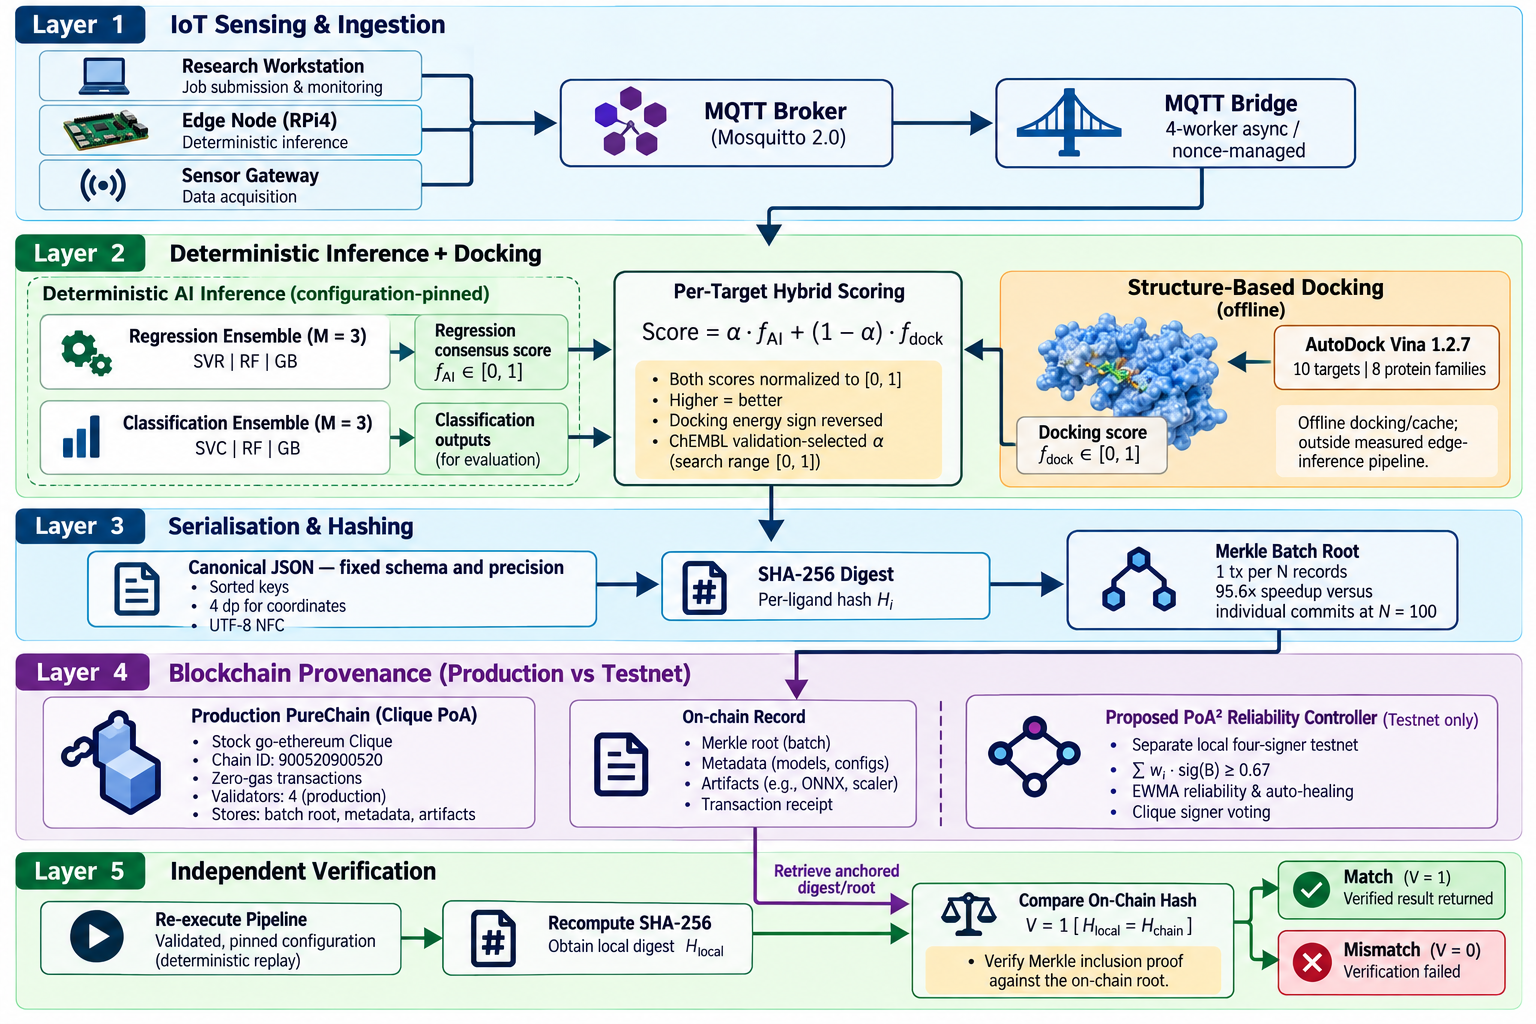
\includegraphics[width=\linewidth]{images/System_Architecture.png}
\end{center}
\textbf{Figure 1 caption.}

\textcolor{blue}{PureProtX architecture.
Production Clique anchoring and independent verification are distinct
from the proposed PoA$^2$ controller evaluated on the local testnet.
The deployed ensemble contains six predictors and one scaler.}
\end{excerpt}

\loc{(b) Pages 8--9: controller deployment scope in Section III-G}
\begin{excerpt}
\mshead{III-G}{Clique Provenance and Proposed PoA$^2$ Control}

\textcolor{blue}{The proposed controller uses reliability observations to request signer-set changes through Clique voting. This behavior is evaluated on the local testnet, not established as a production feature.}

\textcolor{blue}{A violation motivates replacement of a low-reliability signer by a standby through the standard Clique voting interface. The measured local controller uses its configured observation window and threshold; the experiment validates that controller scenario, not a weighted production consensus implementation.}
\end{excerpt}

\loc{(c) Page 17: production validation remains future work}
\begin{excerpt}
\mshead{VI}{Conclusion}

Having validated the gap-condition mechanism through
controlled failure injection on a permissioned testnet
(Section~\mbox  {V-B}), a natural next step
is failure-injection on the production deployment and at
larger signer-set sizes to confirm the recovery envelope
at scale.
\end{excerpt}

\review{1.4}{`Cryptographic auditability essentially free' is too strong. The manuscript reports 41.1\% overhead for one small single-record workload and only negligible overhead under Merkle batching. The conclusion should consistently state that the overhead is negligible under the evaluated batched regime, not universally.}

\reply We agree and have removed ``essentially free'' and
universal negligible-overhead claims. We have also made the distinction
between the measurement regimes explicit. The 41.1\% and 4.9\% figures
are increases relative to compute-only time for separate 1,000-compound
workloads with one anchoring transaction each; they are not measurements
of a one-compound workload.

The separate Merkle experiment reports an amortized anchoring latency.
It does not contain a matched compute-only measurement from which its
percentage overhead can be established. Consequently, we do not retain
``negligible'' as a percentage claim even for that batch experiment. We
withdraw the unsupported $<0.01\%$ value and report the measured latency
reduction instead. The archived $N=100$ CSV gives 19.66~ms per record and
a 95.6-fold anchoring speedup relative to individual commits. R2.2 below
provides the explicit denominator and arithmetic.

\loc{(a) Page 13: qualification of the Merkle overhead claim in Section V-H}
\begin{excerpt}
\mshead{V-H}{Blockchain Anchoring Overhead}

\textcolor{blue}{The separate Merkle experiment at $N{=}100$
has batch anchoring time $T_{\mathrm{anchor}}=1.9663$~s,
or $1000T_{\mathrm{anchor}}/100=19.663$~ms per record.
Amortizing both compute and anchoring by $N$ leaves their
ratio unchanged: relative anchoring overhead would be
$100T_{\mathrm{anchor}}/T_{\mathrm{compute},100}$.
No matched compute-only time for that experiment is recorded,
so a percentage cannot be inferred. Batching lowers per-record anchoring
latency in the evaluated regime; whether its end-to-end
percentage is negligible depends on measured compute time.}
\end{excerpt}

\loc{(b) Page 17: measured latency replaces universal overhead language}
\begin{excerpt}
\mshead{VI}{Conclusion}

\textcolor{blue}{Merkle batch anchoring lowers measured
per-record anchoring latency 95.6-fold at $N{=}100$
(19.66 versus 1,879.94~ms), without establishing a universal
percentage-overhead claim.}
\end{excerpt}

\clearpage
\section*{To Reviewer \#2}
We thank the reviewer for identifying the remaining inconsistencies in the
model inventory, overhead calculation, score orientation, and consensus
labels. We have checked each item against the reported artifacts and
implementation and revised the manuscript as detailed below.

\review{2.1}{Section III-D describes four regression models (SVR, RF, GB, and MLP) and three classification models. However, Tables VIII and IX include the StandardScaler but do not report results for the MLP. Please clarify this discrepancy and, if the MLP is included in the deployed ensemble, provide its corresponding determinism results.}

\reply Thank you for identifying this discrepancy. The
deployed ensemble does not include an MLP. The saved per-target benchmark
records list three regressors (SVR, random forest, and gradient boosting)
and three classifiers; the ONNX manifest contains their six exports plus
one StandardScaler. The former description of four deployed regressors
was incorrect, and the scaler should not have been counted as a predictor.

MLP appears in a separate sklearn training-repeatability test using seeded
synthetic data. That test is not a deployed MLP export and does not provide
MLP cross-runtime or cross-architecture evidence. We have therefore
corrected the ensemble definition and consensus divisor to $M=3$, together
with Algorithm~1, the setup table, architecture, performance description,
abstract, and conclusion. Tables~VIII and IX are now explicitly interpreted
as six predictive models plus a preprocessing scaler. No missing MLP
ONNX result is inferred, and no new MLP experiment is claimed.

The correction is supported by the model-specific entries in
\nolinkurl{experiments/paper_results/revised_results.json}, the export
inventory in \nolinkurl{models/onnx/manifest.json}, and the distinction
from \nolinkurl{tests/test_determinism.py}. The reported saved screening
results already use the three-regressor inventory; this correction does
not introduce a newly trained replacement ensemble.

\loc{(a) Page 6: corrected ensemble and explanation of MLP in Section III-D}
\begin{excerpt}
\mshead{III-D}{Deterministic AI Inference Module}
\mshead{III-D2}{Dual Ensemble Architecture}

The \emph{regression ensemble} comprises \textcolor{blue}{three models: SVR, RF, and GB}, each trained to predict continuous
pIC$_{50}$ values.
The consensus regression prediction is the arithmetic
mean across the $\textcolor{blue}{M{=}3}$ regressors:
\begin{equation}
\hat{y}_{\mathrm{cons}}(\mathbf{x})
  = \frac{1}{M}\sum_{m=1}^{M}\hat{y}_m(\mathbf{x}).
\tag{2}
\end{equation}

\textcolor{blue}{The saved ten-target benchmark results contain these
three regressors, and the deployed ONNX manifest contains their
exports, three classifiers, and one StandardScaler. The scaler is
a preprocessing artifact, not a seventh predictor. MLP was included
only in a separate seeded synthetic-data test of sklearn training
repeatability; it was not part of the reported screening ensemble
or the deployed ONNX pipeline. That test does not establish MLP
cross-runtime or cross-architecture determinism. MLP was therefore removed from the ensemble description. The ONNX tables report six
predictors and one scaler; no MLP determinism claim is made.}
\end{excerpt}

\loc{(b) Page 12: corrected interpretation of the ONNX results inventory}
\begin{excerpt}
\mshead{V-F}{Cross-Platform Determinism via ONNX}

Table~VIII reports on-chain ONNX model hashes,
bitwise determinism across 40~independent inference runs,
and sklearn-to-ONNX concordance for \textcolor{blue}{six predictive models and one scaler}.
\end{excerpt}

\review{2.2}{Table X reports approximately 21 ms per record for Merkle batching at N=100, together with an overhead of less than 0.01\%. The calculation underlying this percentage is not sufficiently clear. Please specify the reference time and calculation method, and ensure that the reported percentage is consistent with the experimental measurements.}

\reply We agree that the previous percentage was not
supported by a specified denominator. We have removed $<0.01\%$ from
Table~X and the abstract, limitations, and conclusion, and added Eq.~(10)
to define percentage overhead relative to the compute-only time for the
same workload. Table~X retains the two measured 1,000-compound cases:
41.1\% for CHEMBL243 and 4.9\% for hERG.

We also reconciled the Merkle figures to the archived scalability CSV,
rather than retaining inconsistent rounded values from the older prose
summary. For $N=100$, the CSV records 1.9663~s for the batch transaction,
19.6628~ms per record, and 187.9944~s for 100 individual commits. The
result is a 95.6-fold anchoring speedup. The previous approximately
21~ms value is replaced by 19.66~ms throughout the revised discussion.

Dividing anchoring time by $N$ does not establish a percentage: compute
time must also refer to the same $N$-record workload. Because the batch
experiment has no matched compute-only reference time, we report its
latency without assigning a percentage overhead. Figure~7 is generated
directly from \nolinkurl{results/scalability_benchmark.csv}; the local
baseline points in Figure~8 come from
\nolinkurl{results/provenance_comparison.csv}. The plotting script checks
the archived arithmetic and records input hashes. The revised figures
are reproduced in excerpt~(c) below, rather than only described in captions. The captions distinguish
one-run chain timings from best-of-five local timings; no additional runs
or confidence intervals are claimed.

\loc{(a) Page 13, Table X: corrected reporting of latency and percentage overhead}
\begin{excerpt}
\mshead{V-H}{Blockchain Anchoring Overhead}
\textbf{Table X caption.}

\textcolor{blue}{Anchoring overhead for 1,000-compound
workloads (five runs; medians). Percentage is the increase
relative to pipeline-only time. The separate $N{=}100$
Merkle experiment reports latency, not a comparable percentage.}

\begin{center}
\begin{tabular}{lrrrr}
\toprule
Target & Pipeline (s) & +Chain (s) & Overhead (s) & Overhead (\%) \\
\midrule
CHEMBL243 & 3.31 & 4.67 & 1.36 & 41.1 \\
CHEMBL240 & 14.34 & 15.03 & 0.70 & 4.9 \\
\bottomrule
\end{tabular}\par\smallskip
\textcolor{blue}{$N{=}100$: 19.66~ms/record; relative overhead not measured.}
\end{center}
\end{excerpt}

\loc{(b) Page 13, Section V-H and Eq. (10): denominator and explicit arithmetic}
\begin{excerpt}
\mshead{V-H}{Blockchain Anchoring Overhead}

\textcolor{blue}{Let $T_0$ be the median pipeline-only time
and $T_1$ the median time with one Clique anchoring transaction
for the same 1,000-compound workload. We report}
\begin{equation}
\textcolor{blue}{\mathrm{Overhead}(\%)=100\,(T_1-T_0)/T_0.}
\tag{10}
\end{equation}
\textcolor{blue}{For CHEMBL243, $100(4.6680-3.3084)/3.3084
=41.1\%$; for hERG, $100(15.0339-14.3361)/14.3361
=4.9\%$ (rounding differences arise from stored precision).
These are increases relative to compute time, not fractions
of total end-to-end time, and each workload has 1,000
compounds rather than one compound.}

\textcolor{blue}{The separate Merkle experiment at $N{=}100$
has batch anchoring time $T_{\mathrm{anchor}}=1.9663$~s,
or $1000T_{\mathrm{anchor}}/100=19.663$~ms per record.
Amortizing both compute and anchoring by $N$ leaves their
ratio unchanged: relative anchoring overhead would be
$100T_{\mathrm{anchor}}/T_{\mathrm{compute},100}$.
No matched compute-only time for that experiment is recorded,
so a percentage cannot be inferred. The previous $<0.01\%$
claim is withdrawn. Batching lowers per-record anchoring
latency in the evaluated regime; whether its end-to-end
percentage is negligible depends on measured compute time.}
\end{excerpt}


\clearpage
\loc{(c) Page 12, Figures 7--8: regenerated plots from the archived measurements}
\begin{excerpt}
\mshead{V-D}{Blockchain Scalability and Merkle Efficiency}
\begin{center}
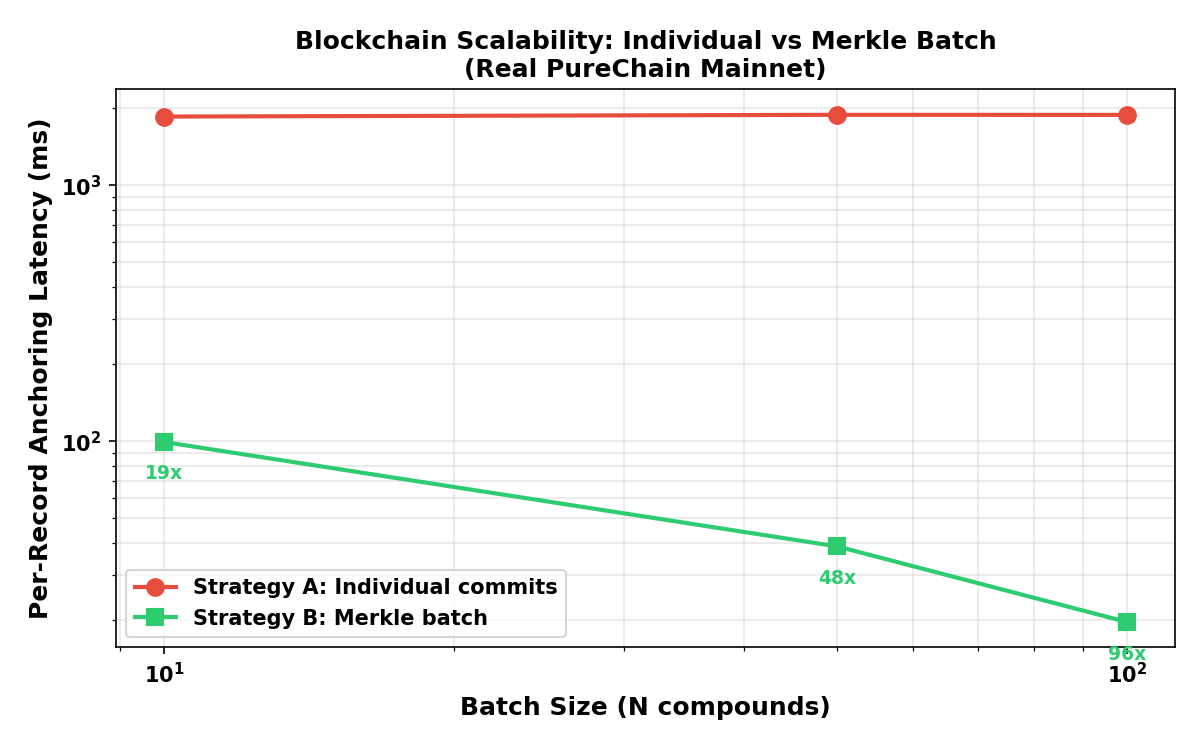
\includegraphics[width=0.86\linewidth]{images/fig_ve_scalability.png}
\end{center}
\textbf{Figure 7.}
\textcolor{blue}{Per-record blockchain anchoring latency versus
batch size (log--log scale), reconciled to the archived
\texttt{results/scalability\_benchmark.csv}. Speedups at
$N{=}10,50,100$ are 18.7, 48.5, and 95.6, respectively.
Batching is already beneficial at the smallest tested size;
the exact crossover below $N{=}10$ was not measured. One archived
run per size is plotted; no error bars are inferred.}

\medskip
\begin{minipage}{\linewidth}
\mshead{V-E}{Comparison with Alternative Provenance Mechanisms}
\begin{center}
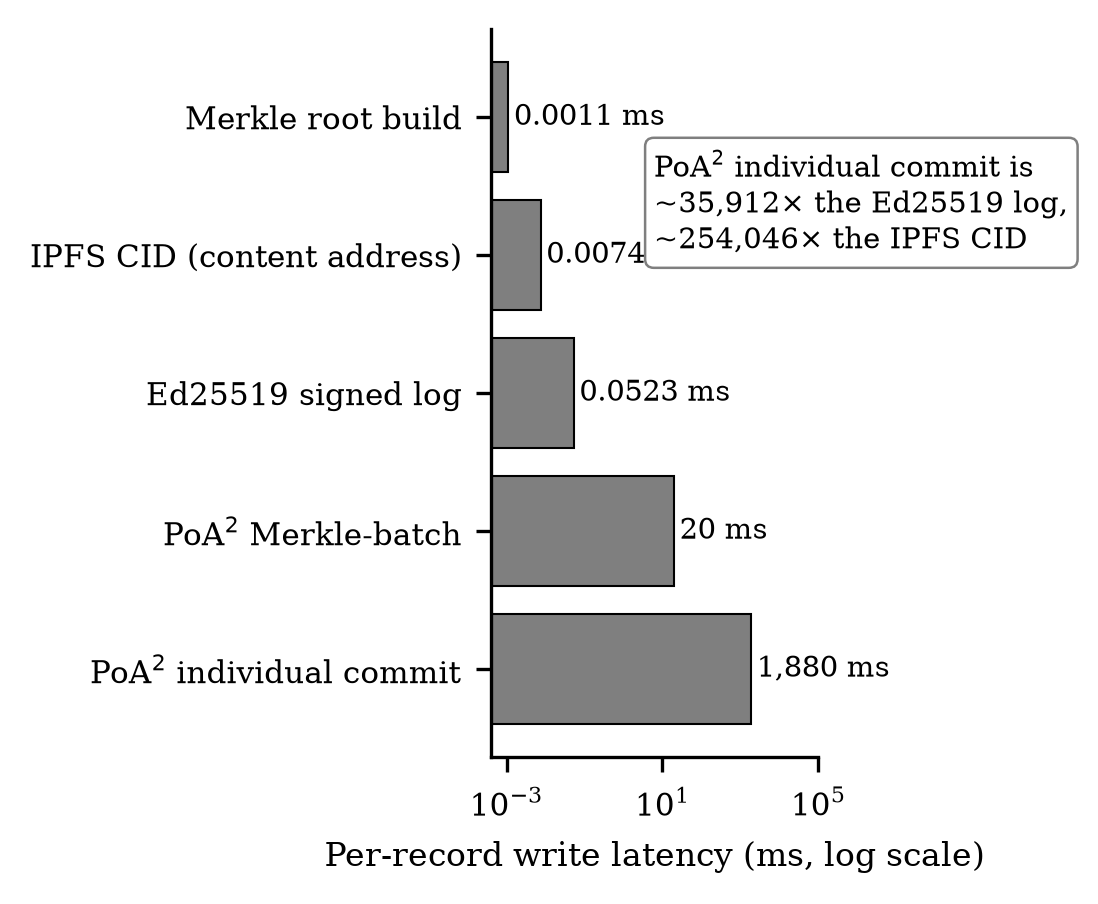
\includegraphics[width=0.86\linewidth]{images/fig3_provenance_cost.png}
\end{center}
\textbf{Figure 8.}
\textcolor{blue}{Per-record write latency of provenance mechanisms
(log scale): Merkle root build, IPFS CID, Ed25519 signed log, and
on-chain anchoring (Merkle-batched and individual commit). Local
mechanisms are microseconds; on-chain anchoring incurs a consensus
round-trip. The on-chain approach is not competitive on cost; its
advantage is the trust model (Table~VII). At $N{=}100$, local
operations use archived best-of-five timings; chain timings come
from the separate archived scalability run. Local CID computation
excludes IPFS persistence and network retrieval.}
\end{minipage}
\end{excerpt}

\review{2.3}{In Eqs. (3)--(4), the normalized docking scores are combined with AI activity scores. Since more negative Vina binding energies generally indicate more favorable binding, whereas higher AI activity scores indicate stronger predicted activity, the score directions require clarification. Please explain the normalization, score orientation, and ranking convention used in the implementation.}

\reply Thank you. The implementation reverses the docking
energy direction before fusion. The previous displayed normalization
omitted that reversal and the bounded mapping, so it did not accurately
describe the code. Equation~(3) now states the negated docking z-score
followed by clipping to $[0,1]$. The regression-consensus AI score uses the
positive z-score with the same bounded mapping. Both terms in Eq.~(4)
therefore increase with predicted activity or favorable binding, and the
final score is ranked in descending order.

We specify that normalization statistics are computed separately within
each target's validation and test score arrays, along with the implemented
short-array and near-zero-variance behavior. We also clarify that the
hybrid benchmark uses normalized regression predictions, while
classification probabilities are evaluated separately; the hybrid AI term
is not an isotonic-calibrated regression probability.

Finally, we correct the former tie-breaking description. The benchmark
metrics order by descending fused score using \texttt{np.argsort(-scores)};
they do not apply the CLI's secondary sorting rule. The separate CLI
utility uses descending consensus score, then ascending raw docking energy,
then lexicographic canonical SMILES. The revised text distinguishes these
paths rather than claiming that the benchmark applies a secondary
regression-pIC$_{50}$ sort. Equations~(3)--(4), the prose, Algorithms~1--3,
and the architecture are aligned with these conventions. These are reporting
corrections, not a new sign change applied to regenerate the screening results.

\loc{(a) Page 7, Section III-E and Eq. (3): orientation and normalization}
\begin{excerpt}
\mshead{III-E}{Docking Module}

\textcolor{blue}{Raw binding energies $\Delta G_i$ are oriented so that
more favorable (more negative) energies yield larger scores. The
implementation applies a negated z-score followed by clipping:}
\begin{equation}
\textcolor{blue}{f_{\mathrm{dock}}(i)
 = \operatorname{clip}_{[0,1]}\!\left(
 \frac{3-(\Delta G_i-\mu_{\Delta G})/\sigma_{\Delta G}}{6}\right).}
\tag{3}
\end{equation}
\textcolor{blue}{For regression predictions $a_i$, the corresponding
AI score is $f_{\mathrm{AI}}(i)=\operatorname{clip}_{[0,1]}
((3+(a_i-\mu_a)/\sigma_a)/6)$. Thus both components are
dimensionless, bounded in $[0,1]$, and higher-is-better. Statistics
are computed separately within each target's validation and test
score arrays in the benchmark code; they are not a pooled
cross-target normalization. For an array with fewer than two entries,
the implementation returns zeros; for a near-zero standard deviation
($<10^{-10}$), it returns 0.5 for every entry.}
\end{excerpt}

\loc{(b) Pages 7--8, Section III-F and Eq. (4): fusion and ranking convention}
\begin{excerpt}
\mshead{III-F}{Hybrid AI--Docking Consensus Fusion}

\textcolor{blue}{Normalized regression-consensus AI scores} $f_{\mathrm{AI}}(i)$ and normalised
docking scores $f_{\mathrm{dock}}(i)$ are fused through
a convex weighting:
\begin{equation}
\mathrm{Score}_{\mathrm{final}}(i)
  = \alpha \, f_{\mathrm{AI}}(i)
  + (1 - \alpha)\, f_{\mathrm{dock}}(i),
\qquad \alpha \in [0, 1].
\tag{4}
\end{equation}
The parameter $\alpha$ is optimised per target on the
validation set by grid search over
$\alpha \in \{0.00, 0.05, \ldots, 1.00\}$ (21~values),
maximising BEDROC.
\textcolor{blue}{The benchmark maximizes the fused score and evaluates
rankings using descending score (\texttt{np.argsort(-scores)}).
It does not apply a secondary regression-pIC$_{50}$ sort. The CLI
ranking utility separately breaks ties by ascending raw docking
energy, then lexicographic canonical SMILES. These are distinct
code paths: the benchmark does not claim that its equal-score
ordering is the CLI's explicit tie-breaking convention.}
\end{excerpt}

\review{2.4}{Section III-G clarifies that the production network uses Clique consensus, with PoA$^2$ operating as a control-layer mechanism. However, the caption of Fig. 2 still describes PoA$^2$ finality based on weighted validator signatures, while Table VI refers to "PoA$^2$ consensus latency." Please consider aligning these descriptions to distinguish the underlying consensus mechanism from the proposed control layer.}

\reply We agree. Figure~2 no longer depicts weighted
validator signatures as production finality. Its production step now
describes transaction submission to Clique, block sealing by an authorized
signer, and waiting for the transaction receipt. The caption explicitly
identifies the approximately two-second quantity as transaction-to-receipt
latency and separates the proposed controller's local-testnet evaluation.

Table~VI is now captioned ``Production PureChain (Clique)
transaction-to-receipt latency (ms),'' and Section~V-B is titled
``Clique Commit Latency and Hash Integrity.'' The accompanying explanation
states that latency is not evidence of weighted-signature PoA$^2$ finality.
Section~III-G likewise distinguishes the production protocol from the
proposed policy equations, as explained under R1.2. We have made the same
distinction in the architecture and abstract to avoid contradictory labels.

\clearpage
\loc{(a) Page 8, Figure 2: corrected description of the production anchoring protocol}
\begin{excerpt}
\mshead{III-G}{Clique Provenance and Proposed PoA$^2$ Control}
\begin{minipage}{\linewidth}
\begin{center}
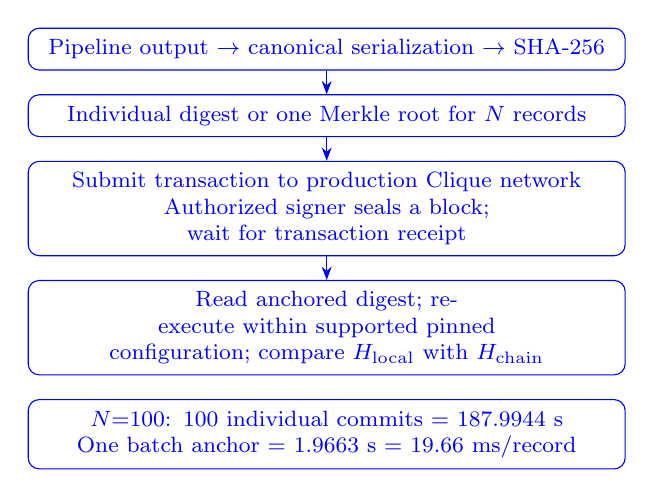
\begin{tikzpicture}[node distance=3mm,
box/.style={draw=blue, rounded corners, align=center, text width=7.3cm,
inner sep=4pt, font=\footnotesize, text=blue}, >=Stealth]
\node[box] (out) {Pipeline output $\rightarrow$ canonical serialization $\rightarrow$ SHA-256};
\node[box, below=of out] (root) {Individual digest or one Merkle root for $N$ records};
\node[box, below=of root] (tx) {Submit transaction to production Clique network\\
Authorized signer seals a block; wait for transaction receipt};
\node[box, below=of tx] (check) {Read anchored digest; re-execute within supported pinned\\
configuration; compare $H_{\mathrm{local}}$ with $H_{\mathrm{chain}}$};
\node[box, below=of check] (cost) {$N{=}100$: 100 individual commits = 187.9944~s\\
One batch anchor = 1.9663~s = 19.66~ms/record};
\foreach \a/\b in {out/root,root/tx,tx/check}
\draw[->,blue] (\a) -- (\b);
\end{tikzpicture}
\end{center}
\textbf{Figure 2 caption.}

\textcolor{blue}{Production
Clique anchoring and digest verification. The ${\sim}2$~s
measurement is transaction-to-receipt latency, not weighted-signature
PoA$^2$ finality. The proposed controller is a separate local-testnet
experiment. Batching amortizes anchoring cost; a percentage overhead
also requires a matched compute-time denominator.}
\end{minipage}
\end{excerpt}

\loc{(b) Page 11, Table VI: corrected measurement label}
\begin{excerpt}
\mshead{V-B}{Clique Commit Latency and Hash Integrity}
\textbf{Table VI caption.}

\textcolor{blue}{Production PureChain (Clique) transaction-to-receipt latency (ms)} and hash
integrity. Active signer set recovered from
block-seal attribution; signer rotation observed (3 of 4 signers in recent blocks).
Blocks~1{,}012{,}544--1{,}012{,}680.
\end{excerpt}

\loc{(c) Page 10: distinction between receipt latency and finality in Section V-B}
\begin{excerpt}
\mshead{V-B}{Clique Commit Latency and Hash Integrity}

\textcolor{blue}{The ${\sim}2$~s median measures transaction submission
to receipt on the production Clique network. The signer evidence
and network configuration establish the validator deployment;
the latency measurement is not evidence of weighted-signature
PoA$^2$ finality.}
\end{excerpt}


\bigskip
We thank the Associate Editor and both reviewers for the careful evaluation.
The changes above correct the remaining claim-scoping and reporting issues
while preserving the distinction between measured evidence and untested
extensions. We hope that the revised manuscript and this point-by-point
response address the remaining concerns.

\medskip
Sincerely,\\
The Authors
\end{document}
